
\documentclass[sigconf]{acmart}

%%
%% \BibTeX command to typeset BibTeX logo in the docs
\AtBeginDocument{%
  \providecommand\BibTeX{{%
    \normalfont B\kern-0.5em{\scshape i\kern-0.25em b}\kern-0.8em\TeX}}}

%% Rights management information.  This information is sent to you
%% when you complete the rights form.  These commands have SAMPLE
%% values in them; it is your responsibility as an author to replace
%% the commands and values with those provided to you when you
%% complete the rights form.
\setcopyright{acmcopyright}
\copyrightyear{2019}
\acmYear{2019}
\acmDOI{}

%% These commands are for a PROCEEDINGS abstract or paper.
%\acmConference[Woodstock '18]{Woodstock '18: ACM Symposium on Neural
%  Gaze Detection}{June 03--05, 2018}{Woodstock, NY}
%\acmBooktitle{Woodstock '18: ACM Symposium on Neural Gaze Detection,
%  June 03--05, 2018, Woodstock, NY}
%\acmPrice{15.00}
%\acmISBN{978-1-4503-9999-9/18/06}


\begin{document}

\title{Comparison of Two Proactive Self-adaptation Methods: PLA and CobRA}


\author{Ben Trovato}
\authornote{Both authors contributed equally to this research.}
\email{trovato@corporation.com}
\orcid{1234-5678-9012}
\author{G.K.M. Tobin}
\authornotemark[1]
\email{webmaster@marysville-ohio.com}
\affiliation{%
  \institution{Institute for Clarity in Documentation}
  \streetaddress{P.O. Box 1212}
  \city{Dublin}
  \state{Ohio}
  \postcode{43017-6221}
}

\author{}
\affiliation{%
  \institution{The Th{\o}rv{\"a}ld Group}
  \streetaddress{1 Th{\o}rv{\"a}ld Circle}
  \city{Hekla}
  \country{Iceland}}
\email{larst@affiliation.org}

\author{}
\affiliation{%
  \institution{Inria Paris-Rocquencourt}
  \city{Rocquencourt}
  \country{France}
}
%\begin{verbatim}
%\bibliographystyle{ACM-Reference-Format}
%\bibliography{acmart}
%\end{verbatim}

\begin{abstract}
Software-intensive systems tend to face more and more uncertainties in running environment, which are difficult to engineer and expensive to consider at design time. Therefore, software systems need to have ability of self-adaptation, to monitor the change of uncertainties and adjust itself dynamically to keep approaching the target. As we consider which methods we should choose to use, we weigh their engineering costs and resulting effects. Currently, there are most advanced two proactive adaptive methods, PLA\cite{pla} and CobRA\cite{cobra}, both adopting ideas from MPC. Gabriel A. Moreno compared the two methods in aspects of development costs and run-time performance\cite{GA}. They spend different efforts on modeling and achieve different effects, but both of them can achieve satisfying adaptation control. In this paper, we followe the experimental senario of G.A and explore the reasons for the similarities and differences between the two on the basis of their work. We find that the open-loop method is difficult to cope with uncertainties such as errors from modeling and prediction. PLA needs to combine feedback to achieve good control effect. We analyze and verify the major differences between them.
\end{abstract}

\begin{CCSXML}
	<ccs2012>
	<concept>
	<concept_id>10011007.10010940.10010971</concept_id>
	<concept_desc>Software and its engineering~Software system structures</concept_desc>
	<concept_significance>300</concept_significance>
	</concept>
	</ccs2012>
\end{CCSXML}

\ccsdesc[300]{Software and its engineering~Software system structures}

\keywords{self-adaptation, PLA, CobRA, model predictive control}

\maketitle

\section{Introduction}
Why do software systems need  capabilities of self-adaptation?
The main reason is that software-intensive systems face a lot of uncertainties while running, such as fluctuant running environment and changing requirements. While in the design time of software systems, considering all those uncertainties is not realizable and needs high cost. However, due to some properties of the software system, we can design an adaptive mechanism to tolerate these uncertainties. The main difference between traditional software engineering and self-adaptation software engineering is that, in traditional software, we will anticipate changes that the software system will face in the future and give the response to them. On the contrary, for self-adaptation, we do not need to design as carefully as possible the solution to all changes that maybe happen, we just need to know some feature of the system, then we can design an adaptation controller to handle these changes according to these features.
Software self-adaptation can be defined as an ability of software system to monitor uncertainties during running and then make adaptive tactics to response to these changes in order to maximize its goal. As shown in figure\ref{fig:mape-k}, software self-adaptation often bases on MAPE-K loop\cite{mape-k}, consisting monitor, analyze, plan, and execute modules sharing a whole knowledge, as shown in figure\ref{fig:mape-k}. The control manager gets measurements from managed system through sensors and then use effectors to execute adaptation tactics.
\begin{figure}[h]
	\centering
	%	\includegraphics[width=\linewidth]{mape-k}
	\caption{MAPE-K architecture}
\end{figure}
However traditional software self-adaptation are reactive, they only make adaptive tactices after changes happened, do not predict what will happen in the future. On the contrary, proactive self-adaptation can predict what will happen in the future, to make tactices ahead of time.
Currently, there are works using control theory to design self-adaptation for software. There is a famous class of control methods in the control field called model predictive control(MPC) to explicitly deal with multivariable systems with constraints. MPC abstracts the system into a linear model of multiple inputs and outputs and then use this model to predict the behavior of systems in the future. It uses a receding horizon to get the optimal control.
Cobra is a typical example of applying control theory to software adaptation. Cobra is a requirement-based approach that employs traditional control theory ideas and regards the system like a black box. It abstracts the system into a simple linear model, modeling requirements into cost function, using feedback to smooth the effects of modeling error and disturbance.
There is a noted self-adaptation method based on ideas of traditional software engineering called PLA. It does not model the system as linear, on the contrary, it regards the system as a white box and constructs precise MDP model to predict the future system and environment. The goal of the system is modeled into revenue function. Then we can use probabilistic model checkers\cite{pmc} to exhaustive all can reach the path and get the solution which can maximize the revenue function.
Although PLA and CobRA have different design ideas and implementation methods, they both adopt MAPE-K loop\cite{mape-k} and employ the idea from MPC. That is, 
1) both use prediction models to predict future behavior. They establish different models for the system and environment.
Cobra models the system as linear and treats the environment as disturbance, while PLA models the system and environment as an integrated MDP and predicts the future environment.
2) adopt the idea of receding horizon to get a optimal solution among the horizon. They compute a series of control actions but only commit the first one.

When we are considering which method to choose, there are some facts that we need to weigh. The most important one is whether the method can handle the problems and achieve the goal of object system. When we model the system, we are simplifying the system, thus inevitably there will have errors between the model and the real system. Unlike in the physical world, which can be modeled by exact mathematical equations, software systems are always more complex to model. Althogh it seems that MDP is more accurate than linear model, but it also exist errors and need more efforts while building. CobRA is not much precise, but it has many theory of guarantees of stability. If we can achieve similar results, obviously we want to use method that needs fewer effort.

Gabriel A. Moreno compared the two methods both in the light of development costs and run-time performance. While the two approaches perform comparably in general, their run-time behavior can be significantly different, both in terms of resource utilization and the ways in which they attempt to maximize performance. Both of them can get fine results after elaborate adjustment of feedback parameters. But they did not analyse the reasons why they achieve the same effect, or the reasons and consequences of their differences.
Therefore, based on their work, we hope to further analyze the reasons why these two methods can achieve the same result, as well as the consequences of their differences under specific scenarios, so as to have a better understand of the applicability of these two methods.

In this work, we first analyze the similarities between the two, and deduce the reasons why the two can achieve similar effects from the perspective of their decision-making process. Then, we analyzed the differences between the two from three aspects, including the three aspects of 1)modeling environment, 2)asymmetric latency and 3)regular terms for optimization. We theoretically analyzed the reasons and effects of the differences, and use the same experiment senario as G.A\cite{GA} to verify our conjecture through experiments.

In the remainder of the paper, Section II presents the adaptation scenario we used. Section III provides an overview of CobRA and PLA both on design and implementation. Next, Section IV details the reasons for their similarities. Section V describes three different aspects of CobRA and PLA. Finally, Section VI presents our conclusions and directions for future research.
\section{adaptation senario}

Based on G.A's work, we carry out our comparison on the RUBiS system\cite{rubis}, an widely used open-source application for evaluation of self-adaption and cloud computing\cite{rubis-1},\cite{rubis-2}. To enable replicating experiments with the same conditions under control for the two approaches, avoiding unexpected fluctuation and uncertainties during real systems running, we ran our experiments on a simulated system of RUBiS, which is named SWIM\cite{swim}.

RUBiS system consists of a load-balancer, a web server tier and a database tier. Clients use browsers to send requests to the server. Load balancer distributes requests among servers following a round-robin policy. Servers access the database to obtain the data required to render the dynamic content of the page.
Figure \ref{fig:rubis} shows the architecture of RUBiS system. 
\begin{figure}[h]
	\centering
	%	
\includegraphics[width=\linewidth]{rubis}
	\caption{Architecture of RUBiS}
\end{figure}
We introduce the characteristics of RUBiS system from the three aspects of uncertainties, tactics and utility:
\begin{itemize}
	\item {\verb|Uncertainties|}:
	
	The main uncertainties of RUBiS system, which is need to sovled by the adaptation controller, can be divided into three categories:
	\begin{enumerate}
		\item {\verb|Environment|} For RUBiS system, the only relevant property of the running environment that we consider is the arriving requests on the system. If the arrival rate of requests increases suddenly, the system need more resource to handle them.
		\item {\verb|Latency of adding a server|} For RUBiS system, there is a period time that before a new server can start working. We call it \textit{latency} of adding servers. 
		\item {\verb|How long it needs to process a request|} That is the service time in RUBiS system depending on the performance of the system and the nature of the specific requests.
	\end{enumerate}
	\item {\verb|Tactics|}: 
	For RUBiS system, the main uncertainty that self-adaptation want to handle is the uncertain environment. RUBiS system can execute two types of tactics to adjust itself in order to deal with uncertainties:
	\begin{itemize}
		\item {\verb|Add/remove server|} There is a delay in adding a server, which we call it latency, whereas removing a server can be consider as no latency, because the latency for removing a server is negligible.
		\item  {\verb|Increase/decrease dimmer value|} RUBiS system follows the brownout paradigm\cite{brownout}, which can response to a request includes mandatory content and optional content. The dimmer parameter indicates the proportion of a request including optional content(value between $[0,1]$).
	\end{itemize}
	\item {\verb|Utility|}:
	The goal of the target system can be described as two functional and three non-functional requirements. Functional requirements are tasks of the system, whereas we capture non-functional requirements formally in a utility function that enables us to quantify their satisfaction. The utility function is modeled as follows:
	\begin{equation}
	\begin{aligned}
	U_{\tau}=\left\{
	\begin{array}{rcl}
	U_{R}+U_{C} & & { r\leq T\wedge U_{R}=U_{R}^{*}} \\
	U_{R} & & {r\leq T\wedge U_{R}<U_{R}^{*}}\\
	\tau min(0,\alpha-\kappa)R_{O} & & {r>T}\\
	\end{array} \right.
	\end{aligned}
	\end{equation}
	\begin{itemize}
		\item utility associated with \textit{cost }per time interval:
		\begin{equation}
		U_{C}=\tau \cdot c\cdot (s^{*}-s)
		\end{equation}
		\item utility associated with revenue per time interval:
		\begin{equation}
		U_{R}=\tau \cdot \alpha \cdot (d\cdot R_{O}+(1-d)\cdot R_{M})
		\end{equation}
		where $\tau$ is the length of the interval, $\alpha$ is the average request rate, and \textit{d} is dimmer value. $R_{M}$ and $R_{O}$ are the rewards for serving a request with mandatory and optional content,respectively.
	\end{itemize}
	The most important requirement is keeping the response time $r$ below the threshold $T$. The second one is the target system shall provide high quality of service, which is described by dimmer value $d$. The third one is that the target system shall use little number of servers $s$ to operate under low cost. The whole goal is to get higher revenue while generate lower cost.
\end{itemize}
\section{Two proactive self-adaptaion methods: PLA and CobRA}
Both of the two approach are based on MPC\cite{mpc} idea. To achieve proactive features, both of them consider an adaptation \textit{horizon}, which is some periods in the future. Decisions are made not only based on historical circumstances and current measurements, but also on the predicted future. We discretizes the execution of adaptation decison in periods of $\tau$, and the system and environment behavior in the adaptation horizon is presented by prediction models. For our senario, we first define the target problems to be solved by the adaptive methods. 
\begin{itemize}
	\item {\verb|Adaptation uncertainties|}:
	There are two kinds of uncertainties faced by self-adaptation controller. One is the uncertainty to be solved by the adaptive system, which is the external uncertainty. For RUBiS system, it includes the arriving rate of requests, the delay of how long it takes to start a server, and how long it takes to process a request, etc. The other type is the uncertainties faced in the design of controller. One is that there will be errors between the actual system and the model, as well as in the PLA's environmental prediction and data measurement.
	The solution of the first kind of uncertain reflects the control effect of the adaptive method itself.
	Tolerance for the second type of uncertainty reflects the properties of the controller, such as stability, which can be measured by SASO properties\cite{saso}.
	The second type of uncertainty will seriously affect the realization of the the non-functional requirements . In order to ensure the completion of their control goals, excellent controllers need to have the ability to tolerance uncertainties.
	\item {\verb|Adaptation goal|}:
	The goal of adaption controller is to decide how to adapt to maximize the utility the system will accrue over the look-ahead horizon, with the monitoring, analysis, planning and executing part, dealing with the influence of uncertainties. And we expect the controller performance is robust, having the ability of resisting disturbance.
\end{itemize}
We describe PLA and CobRA in terms of design details and implementation.
\subsection{PLA}
The key idea of PLA is to let the adaptation decision underspecified through nondeterminism and construct a formal model for the adaptive system and then have the probabilistic model checker resolve the nondeterministic choices to find the way that maximize the accumulated utility over the horizon\cite{pla}. System behavior in the adaptation horizon is predicted by modeling The system into a MDP\cite{mdp}, which uses state changes to express the execution of adaptation tactics. 

The future environment is be modeled as a DTMC in which the random variable representing the state of the environment has one change at each evaluation period $\tau$. PLA uses an autoregresive (AR) time series predictor\cite{ar}, such as RPS toolkit\cite{rps}, to predict future environment, which requires that the changes of environment should be predictable and regular. Because the predictor can provide the variance of the estimation, PLA uses the Extended Pearson-Tukey (EP-T)\cite{ept} threepoint approximation to construct probability trees for decision making. As shown in figure\ref{fig:envtree}, the root $e_{0}$ of the tree is currunt environment, and $e_{1}$ is the estimation distribution of environment in next period with probabilities 0.185, 0.630, and 0.185, respectively.
\begin{figure}[h]
	\centering
	%	
\includegraphics[width=\linewidth]{envtree}
	\caption{Probability Tree of Environment}
\end{figure}
Unfortunately, there will be large errors in the prediction of future environment. In addition, sudden fluctuations cannot be predicted, which will have a great impact on decision-making. This will be analyzed in detail later. Finally, the system and environment are built into a whole MDP model, and the goals of the system are constructed into the form of utiity function. 
The models of the system and environment are stored in \textit{knowledge}. At every beginning of adaptation period, monitor gets measurements from the system and then update the models. Because of the round-robin strategy of RUBiS, we use LPS queuing theory model\cite{lps} to calculate the response time of the system.
We can use a probabilistic model checker\cite{pmd}, such as PRISM\cite{prism} to analyze the model, verify the attributes, exhaust all paths and find a strategy to maximize the utility function. 

In design time, PLA need plenty of effort to build an accurate model of the environment and the target system. It is a feed-forward method, thus the result largely depend on modeling.

\subsection{CobRA}
CobRA adopts more ideas of control theory.
The non-functional requirements of RUBiS system are captured by the softgoals: High Performance, Low Cost, and High Optional Content Availability.
CobRA refers to adaptation goals as \textit{indicators}, for RUBiS system, they are: \textit{r} for average response time of requests, \textit{s} for number of servers and \textit{d} for dimmer value, and constitute the system's output. The parameters of the system that can be tuned in order to fulfil its goals are called \textit{control parameters}. For RUBiS system, \textit{control parameters} are the number of servers \textit{s} and the dimmer value \textit{d}, which constitute the system's input. As well as PLA, CobRA discretizes the execution timeline in adaptation periods of $\tau$, and solves the adaptation decision problem at the start of every period.

CobRA abstracts the relationship between the input and output of the system into a simple linear model. The model represents affects of control parameters to indicators over time. We can use a discrete-time linear dynamic model to describe the system behavior at the k-th decision period.

\begin{equation}
\left\{
\begin{array}{rcl}
x(k+1)=A\cdot x(k)+B\cdot u(k)\\
y(k)=C\cdot x(k)+D\cdot a(k)\\
\end{array} \right.
\end{equation}
where $x$ is the state of the system, $u$ is the set of control parameters, $y$ is the set of indicators and $a(k)$ is the average arrival rate of requests at the k-th decision period.

For the uncertain environment, CobRA does not predict future environment, instead, it treats the environment as disturbance to the system. In our scenario, the environment is uncertain arrival rate of requests \textit{a}, that is used as a feedforward signal. The effect of environment's uncertainty is reflected by Kalman Filter on the system's states.

CobRA is requirement-based, fot RUBiS system, the system's goal can be described as three output variables: the number of servers \textit{s}, the dimmer value \textit{d}, and the average response time of requests \textit{r}.
The goal of the system is that each indicator should be close to its target value, and the goal of the system is designed into the form of cost-function. CobRA make decisions by modifying the value of the control variables.
\begin{equation}
\begin{aligned}
&J_{k}=\sum_{i=1}^H [y_{k+i}^o -y_{k+i}]^TQ_{i}[y_{k+i}^o -y_{k+i}] \\
&+[\Delta u_{k+i-1}]^T P_{i}[\Delta u_{k+i-1}]
\end{aligned}
\end{equation}
where $Q_{i}$ and $P_{i}$ are symmetric positive semi-definite wetghting matrics. $Q_i$ means that when not all the goals can be achieved, the controller will prefer the satisfaction of the goals with high weights. $P_i$ means that the controller want to change the control parameters frequently with smaller weight. $y_{k+i}^o$ are setpoints of indicator i, which means the goal value of this indicator. 

The optimization problem can be definited as follows:
\begin{equation}
\begin{aligned}
&minimize_{\Delta u_{k+i-1}}\qquad J_t \\
&subject\quad to \qquad u_{min}\leq u_{k+i-1}\leq u_{max},\\
&{\Delta u_{min}}\leq{ \Delta u_{k+i-1}}\leq {\Delta u_{max}},\\
&\tilde{x_{k+i}}=\tilde{A}\cdot \tilde{x_{k+i-1}}+\tilde{B}\cdot \Delta u_{k+i-1}, \\
&y_{k+i-1}=\tilde{C}\cdot \tilde{x_{k+i-1}},\\
&\quad i=1,...,H,\\
&x_{k}=x(k)
\end{aligned}
\end{equation}
CobRA makes adaptation decisions to keep indicators as close to setpoints as possible. The control scheme is represented as figure\ref{fig:cobra}
\begin{figure}[h]
	\centering
	%	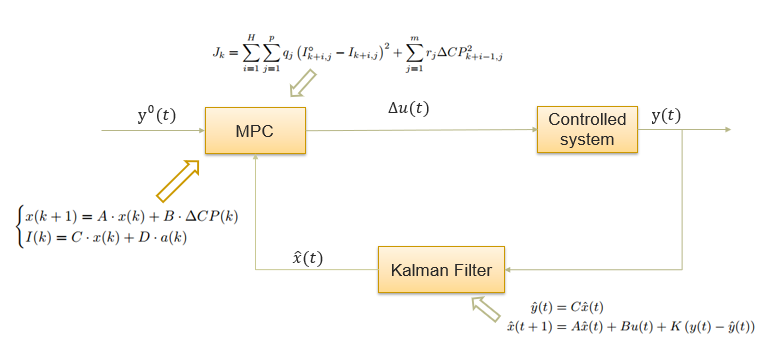
\includegraphics[width=\linewidth]{cobra}
	\caption{Control Scheme of CobRA}
\end{figure}
 
\section{Similarities}
Although there are great differences between the two methods in terms of design and implementation, both of them can achieve a reasonable control effect similarly. In the work of G.A\cite{GA}, they compared the performance of the two methods, including adaptive control performance and SASO property\cite{saso}. They compared the utility value of the two methods when they are running and concluded that in different scenarios, the two methods have different control effects on dimmer value and server numbers, but for the same scenario, they ultimately achieve similar utility value. We would like to explore the reasons why they can achieve similar control effects under so many differences. 

The decision-making of these two methods are actually two different constrained optimization problems. For convenience of comparison, we express the control action in the form of "augmented velocity form" of control variables, similar to the description in CobRA. For PLA, it is a linear constrained optimization problem. Maximizing utility can be transformed into minimizing the minus of utility, $u$, which can be expressed as follows:
\begin{equation}
\begin{aligned}
&min\quad U=(s_0+\Delta s)*cost-\dfrac{d_0+\Delta d}{a}*(N-L), \\
s.t.\quad &r\leq T,\\
&-0.1\leq \Delta d\leq 0.1, -1\leq \Delta s\leq 1,\\
&0\leq d_0+\Delta d\leq 1,1\leq s_0+\Delta s\leq 3
\end{aligned}
\end{equation}
Under the current measured system configuration and environment state, that is, known $s_0$, $d_0$ and $a$, by solving this optimization problem, we can get the control increment, $\Delta s$ and $\Delta d$to minimize $u$ while satisfying their constraints. Because of PLA's prediction for environment, in every decision period in the horizon, $a$ is the prediction of future prediction, which is different from CobRA following.

For CobRA, it is a quadratic constrained optimization problem. In control theory, it is most common to use quardratic performance indices to achieve smooth and robust control results. It can be described as:
\begin{equation}
\begin{aligned}
&min\quad J=(r'-r^o)^2∗Q_{33}+(s_0+\Delta s-s^o )^2∗Q_{11}\\
&+(d_0+\Delta d-d^o)^2∗Q_{22}+(\Delta s)^{2}∗R_{11}+(\Delta d)^2∗R_{22}\\
s.t.\quad &-0.1\leq \Delta d\leq 0.1, -1\leq \Delta s\leq 1,\\
&0\leq d_0+\Delta d\leq 1,1\leq s_0+\Delta s\leq 3
\end{aligned}
\end{equation}
In the current measured system configuration and environment state, CobRA hopes to find the control increments that can minimize $J$ and satisfy the constraints at the same time. The environment state $a$ here is the measured environmental value. However, CobRA will use Kalman Filter to adjust the system state to reflect the fluctuation of environment.
 
Obviously they are two different constrained optimization problems, can they get the same solution under the same input?
We can obtain KKT conditions for two problems through Lagrangian multiplier method. The important factor influencing CobRA's decision making is the setting of parameters in the cost-function and system model, which was also argued in the work of GA.
CobRA relies heavily on the value of weight matrix, feedback adjustment parameters and setpoint value, which determine the optimal solution of cost-function.
In our scenario, if we want to optimize the solution of CobRA to maximize the utility of the system, we think that the values of setpoints, $s^o$, $d^o$ and $rt^o$, should change in every decision period. However, in many related works, setpoints are rarely changed, and are always set to fixed values. Moreover, we think it is not reasonable to set setpoint $r^o$ to 0, because the response time of requests approaching 0 does not make the system optimal, but approaches a value below the threshold of the response time.
Also, it is not reasonable to set $rt^o$ as the threshold, because it is impossible for each indicator to reach the target value in many cases. Instead, it fluctuates around the target value according to the weigh matrixs. However, the threshold value of response time seriously determines the revenue calculation of the system. Once the threshold value is exceeded, the revenue will be punished directly, so we should choose a more appropriate value between $0$ and the threshold value as the setpoint of response time.

We assume that PLA obtaines a optimal solution ,$s_0$ and $d_0$, to the problem in a given state. We set the setpoint in CobRA of $s$ and $d$ to $s_0+\Delta s$ and $d_0+\Delta d$. 
\begin{equation}
\begin{aligned}
&min\quad J=(s_0+\Delta s-s^o)^2 Q_(11)+(d_0+\Delta d-d^o)^2 Q_(22)\\
&+(r'-r^o)^2 Q_(33)+\Delta s^2 R_(11)+\Delta d^2 R_(22)+\alpha _1(-\Delta d-0.1)\\
&+\alpha _2(\Delta d-0.1)+\alpha _3(-d_0-\Delta d)+\alpha _4(d_0+\Delta d-1)\\
&+\alpha _5(-\Delta s-1)+\alpha _6(\Delta s-1)+\alpha _7(-s_0-\Delta s+1)\\&+\alpha _8(s_0+\Delta s-3)
\end{aligned}
\end{equation}
where
\begin{equation}
\begin{aligned}
&r'=k_1 *(s_0+\Delta s)+k_2 *(d_0+\Delta d)+k_3*a,\\
&\alpha _1,\alpha _2,\alpha _3,\alpha _4,\alpha _5,\alpha _6,\alpha _7,\alpha _8\geq 0
\end{aligned}
\end{equation}
We can get the KKT optimality conditions as follows:
\begin{equation}
\begin{aligned}
&2(s_0+\Delta s-s^o)Q_(11)+2k_1 (r'-r^o)Q_(33)\\
&+2\Delta s R_(11)-\alpha _5+\alpha _6-\alpha _7+\alpha _8=0,\\
&2(d_0+\Delta d-d^o) Q_(22)+2k_2 (r'-r^o)Q_(33)\\
&+2\Delta d R_(22)-\alpha _1+\alpha _2-\alpha _3+\alpha _4=0,\\
&\alpha _1(-\Delta d-0.1)=0,\alpha _2(\Delta d-0.1)=0,\\
&\alpha _3(-d_0-\Delta d)=0,\alpha _4(d_0+\Delta d-1)=0,\\
&\alpha _5(-\Delta s-1)=0,\alpha _6(\Delta s-1)=0,\\
&\alpha _7(-s_0-\Delta s+1)=0,\alpha _8(s_0+\Delta s-3)=0
\end{aligned}
\end{equation}
It needs to be discussed separately when $s_0, \Delta s, d_0 and \Delta d$ take different values. But we can get the conclusion when $rt^o$ and weight matrixs Q, R meet some specific relationships, the optimization solution of CobRA can also get the same solution as PLA.
In fact, the constraints on the variation of the control parameters are not the same here. The reason is that CobRA applies to continuous parameters while PLA applies to discrete parameters.
In RUBiS system, before executing the tactic, we need to discretize the continuous variables obtained by CobRA, and the discretization process may produce the phenomenon that the obtained values are not exactly the same, but they can reach the same result after discretization.

Through the above analysis, we can know that under the same initial state, the two can obtain similar control decision results.
However, at run time, it is difficult for them to implement the same control input for each decision, due to their different abstraction of the model and prediction for the environment.
PLA is an open-loop method in terms of architecture, that is, the control effect at one decision period does not affect the decision making at the next period.
However, they can still achieve similar effects because PLA also uses feedback in the implementation.
In the work of GA, it is proposed that in the process of implementation, Kalman Filter is used to dynamically adjust the value of service rate according to the differences between the calculated value and the real value of response time. In fact, it adjusts the servicetime of the system, which is the value describing the service capability of the system and should not be adjusted with the change of workload. So this adjustment is just to make the model more realistic, which is not much reasonable.
There are many errors in PLA. First, it is inevitable that there will be errors in environment prediction. Second, in implementation, PLA uses LPS queuing  model to simulate the system modeling, LPS queuing theory model is very accord with RUBiS system service mode. However, queuing theory models calculate system parameter values under steady state, but during running, as a result of the load fluctuation, systems are difficult to achieve stable states.
Therefore, there will be a certain error between the calculated value of queuing model and the actual response time of the system. As the system is exponential, when the critical value is triggered, the difference will be significant, which will affect PLA to make correct decisions.
\begin{figure}[h]
	\centering
%%	
\includegraphics[width=\linewidth]{rtcompare}
	\caption{Errors in response time calcultation}
\end{figure}
In order to explore the influence of the feedback, we remove the feedback in PLA.
figure\ref{fig:rtcompare} shows the actual response time and the calculation of response time under ClarkNet, there is a certain gap between leads to PLA method failed to under the condition of the response time is more than threshold make reasonable decisions. In figure\ref{fig:planokalman}, we can see that there are several period the response time is exceeding the threshold but pla does not make adaptation decisions to handle it. That is because the response time calculated by the queuing theory model is below the threshold value. PLA makes decisions based on the calculated value, and it is determined that no control decisions need to be made at this moment.
\begin{figure}[h]
	\centering
	
\includegraphics[width=\linewidth]{planokalman}
	\caption{PLA without feedback}
\end{figure}

We can get the conclusion that PLA and CobRA are facing a lot of errors at run time, PLA can tolerates errors because it introduces feedback into the implementation. When there are inevitable errors in prediction and model, the only way to solve this uncertainty is to use feedback.
\section{Differences}
By analyzing the design ideas of PLA  and CobRA, we can obtain some differences between them, which are mainly described in table \ref{tab:differences}.
\begin{table*}
	\caption{Differences between PLA and CobRA}
	\label{tab:differences}
	\begin{tabular}{ccl}
		%\newcommand{\tabincell}[2]{\begin{tabular}{@{}#1@{}}#2\end{tabular}}
		\toprule
		Features&PLA&CobRA\\
		\midrule
		Method & Architecture-based& Requirement-based\\
		Model for Environment & Predict and model to DTMC
		& Do not predict and regard as disturbance 
		\\
		Feedback & Open-loop
		 & Closed-loop\\
		Control  & tactics& Control parameter values
		\\
		Discrete or Continuous&discrete&Continuous\\
		Unsymmetric Latency&Model the unsymmetric latency&Can not model the unsymmetric latency
		\\
		Total Model&Non-linear MDP Model&Linear Dynamic Model\\
		Optimization&Utility function&System goals following boolean AND/OR semantics\\
		
		\bottomrule
	\end{tabular}
\end{table*}
In GA's work, it has been analyzed that there are significant differences between the two in those aspects: artifact, prerequisite and specification.
But we want to talk more about the context in which these differences make a significant difference, and how these differences affect the control effect.
We discuss the differences from three aspects. They are the modeling of asymmetric delay, the difference of environment prediction, discuss how much prediction plays a role, and the constraint of regular term. We followed G.A's parameter settings and workloads, worldcup\cite{worldcup} and clarknet\cite{clarknet}. 
\subsection{Prediction of Environment}
One of the most significant differences between the PLA and CobRA is that they model the environment differently.
PLA regards the environment as an important uncertainty factor of the system and the target problem of the adaptive control.
PLA believes that the future environment will change. At the beginning of every decision period, current and historical environmental data can be obtained. PLA uses known data to predict the future environment in the horizon, and predicts the future response time according to the predicted value of the environment, so as to make decisions.
CobRA regards the environment as one of the disturbances of the system and does not predict the environment, but as a direct component adding to the state space function.
Kalman Filter is used to achieve smoothing and feedback, so as to reflect the influence of the environment to the state change of the system.
Both of the two methods take account of fluctuations in the environment, but they respond in different ways, one using prediction and the other using feedback.

Theoretically, the feedback is one-step slower than the current state, but prediction also have errors.
In addition, although the two methods are different, they have the same assumption for the environment, which requires the environment to change slowly and regularly, so as to ensure that the prediction error is tolerable, and the feedback adjustment can produce appropriate effects.
\ref{fig:planopre}PLA still needs to use feedback to make up for the prediction error, although it makes prediction to the environment. If PLA does not predict the future environment, but only uses the feedback correction system state to reflect the changes of the environment, this is very similar to CobRA. We discuss whether similar results can be produced, so as to determine whether the prediction is necessary, and try to propose improved PLA and CobRA
\begin{figure}[h]
	\centering
		
\includegraphics[width=\linewidth]{planopre}
	\caption{PLA without prediction for environment VS prediction}
\end{figure}

我们在两个负载下分别进行了实验,统计了实验数据以及收益值进行比较。可以发现,如果没有预测,仅仅靠反馈,实验结果取决于反馈的力度,也就是卡尔曼滤波参数的设置,我们同样可以调优调得一个很不错的结果。其实,预测在PLA里面不是必须的,因为预测的误差依旧需要靠反馈来弥补。
我们也有考虑在cobra中引入对环境的预测,是不是控制效果会更好一些。但是实验证明不是很明显。原因在于cobra假设环境是平稳变化的,因此卡尔曼滤波足以应对平稳变化的环境,加入预测不是很必要。
We experiment with two wrokloads respectively, and compared the indicators and utility values.
It can be found that if there is no prediction and only relying on the feedback, the experimental results depend on the feedback strength, that is, the Kalman Filter parameter setting, we can also tune a very good result.
In fact, prediction is not necessary in PLA, because the error of prediction still needs to be compensated by feedback.

We are also considering whether it would be better to introduce environmental prediction to CobRA.
But the experimental results are not so noteworthy.
The reason for this is that CobRA assumes that the environment is stable, so Kalman Filter is sufficient to deal with the stable environment.
\subsection{Asymmetric Latency}
Although RUBiS system is relatively simple, it has some features that are worth exploring for similarities and differences between the two methods.
In RUBiS system, for the couple of decisions about server numbers, there is a certain latency when increasing the number of servers, but reducing the number of servers can be regarded as no delay. This is an asymmetric latency with a control parameter.
PLA models each decision and the asymmetric latency is well described by the MDP model.
However, in CobRA, asymmetric delay was not taken into account. CobRA's model considers that the delay was symmetric, that is, after modeling the latency of adding server, removing server was also considered having latency.
This will cause CobRA to make the decision to reduce the server in advance, and increase dimmer to compensate when reducing the server, reflecting the characteristics of concurrent.

We assume that the linear model of the system is obtained through system identification:
\begin{equation}
	r=k_1 *s+k_2 *d+k_3*a
\end{equation}
To translate this into a state space model, we use the state matrix $A$ to reflect the latency of adding server. The matrixs in the state space model of(4) are:
$A={\left[\begin{array}{ccc}
	0&0&0\\
	1&0&0\\
	0&0&0\\
	\end{array}
	\right]
}$, $B={\left[\begin{array}{ccc}
1&0\\0&0\\
0&1\\
\end{array}
\right]}$, $C={\left[\begin{array}{ccc}
1&0&0\\
0&0&1\\
0&k_1&k_2\\
\end{array}
\right]
}$, $D={\left[\begin{array}{ccc}
0\\
0\\
k_3\\
\end{array}
\right]
}$.
That is: 
\begin{equation}
r(k)=k_1 *s(k-2)+k_2 *d(k-1)+k_3*a(k-1)
\end{equation}
Under this model, it can be found that at time $k$, the number of servers used is the measured value at time $k-2$, leading to a delay in removing servers.
Therefore, when the decision is made to reduce the number of servers, in fact, the number of servers immediately decreases, which will lead to an error in the calculation of response time and affect the decision-making of the system.

At this point, CobRA decides that it needs to reduce the number of servers (why?
As the system described in the model has a delay in reducing the number of servers, the controller considers that the number of servers cannot be reduced during this period. In order to maximize the revenue, it will choose to increase dimmer to compensate for the impact on the revenue during this period.
This may cause the actual response time to exceed the threshold and, if not, reduce the load fluctuations the system can withstand.

当latency有大有小,影响是否一样?

However, in the field of control, it has been proved that the MPC method can tolerate the imprecision of the model to a certain extent due to the function of feedback regulation.
We ran an experiment to verify this conclusion.
One way to modify CobRA to allow for asymmetric delays is to use a dual model.
We can design another system model to be used when removing the server, and the state matrix A is the matrix that does not reflect the delay, $A={\left[\begin{array}{ccc}
	0&0&0\\
	0&0&0\\
	0&0&0\\
	\end{array}
	\right]
}$, While optimizing the solution, the corresponding model is used when the decision of reducing the server occurs.
\subsection{regularization}
In CobRA's cost-funtion, it has constraints on the actuation of control parameters, prefer as little change as possible according to the weight matrixs. However, PLA does not constraint on the actuations. In addition to the expected value of indicators, it is also clear that users are concerned about actuation of control parameters. Frequently actuating the control parameters will cause expensive costs or specific efforts. Consequently, CobRA takes the input signal into account. However, for our experiment, RUBiS is just able to adjust discretely and servers are only allowed to increase one at a time, the difference between PLA and CobRA is not so much serious. We can regard it as when there are more than one ways to achieve maximun utility, CobRA prefer to choose the one with less actuation of control parameters while PLA will choose at random. When there can be huge adjustments, it will make a big difference.

\section{conclusion}
我们在GA工作的基础上,分析对比了PLA 和cobra两种方法的相同点与不同点。在GA的工作中提出二者能够实现相似的控制效果,我们探究了其原因,发现PLA解决预测误差和模型误差的方法是使用反馈调节。由于PLA是一个开环的方法,当PLA方法没有反馈调节的作用时,无法解决因为建模和预测带来的误差。其次我们主要从三个方面分析了二者的不同之处,首先,PLA可以建模非对称延迟,而cobra没有建模非对称延迟,但是控制领域有研究证明,mpc的方法可以容忍一定程度上的模型不精确性。当延迟超过多少时,会对cobra方法的控制性能产生较大影响。第二个方面是二者对环境的建模不同,PLA对未来的环境进行预测,而cobra则将环境视为扰动,不进行预测,而是利用反馈将环境的影响体现到状态上。由于二者都有反馈,我们讨论了PLA中预测的必要性。发现其实在反馈调节的作用下,预测的作用不是很明显。第三点是cobra对控制量的变化量有约束。这当在什么情况下会使二者产生较为明显的区别。
在未来的工作中,我很希望去定量地衡量,得出更一般性的结论。
Based on the work of GA, we analyzed and compared the similarities and differences between the PLA and CobRA.
In the work of GA, it was proposed that the two could achieve similar control effects. We explored the reasons and found that the PLA's solution to the prediction error and model error was feedback adjustment.
As PLA is an open-loop method, the errors caused by modeling and prediction cannot be solved when PLA method has no feedback regulating effect.
Secondly, we analyzed the differences between the two in three aspects. Firstly, PLA can model asymmetric latency of adding servers, while CobRA does not model that. However, studies in the control field have proved that the MPC method can tolerate a certain degree of model inaccuracy.
When the latency is larger than that, the control performance of CobRA will be greatly affected.
The second aspect is the difference in environment modeling between the two methods. PLA predicts the future environment, while CobRA regards the environment as disturbance and does not predict, but reflects the impact of the environment to the state through feedback.
With feedback from both, we discussed the necessity of prediction in the PLA.
It was found that the effect of prediction was not obvious under the effect of feedback.
The third point is that CobRA is limited in how much you can control.
Under what circumstances does this make a clear distinction between the two.
In my future work, I hope to make quantitative measurement and draw more general conclusions.
\bibliographystyle{ACM-Reference-Format}
\bibliography{acmart}
\end{document}
\endinput

